% =====================================================================
%  DA-ZVAD — Project report, IEEE conference format (IEEEtran)
%  Covers the whole project through Phase 3 (October 2026).
%
%  Overleaf: upload this file, references.bib, dazvad_architecture.pdf and
%  the figure PDFs listed in FIGURES below (flat, or in a figures/ folder).
%  Compile with pdfLaTeX; run BibTeX, then pdfLaTeX twice.
%
%  FIGURES: dazvad_architecture, fig_dataset_samples, fig_chart_sweep,
%           fig_chart_within_view, fig_chart_per_camera, fig_chart_ucf_crime
%
%  Every number here is the same as in main.tex (the full living document)
%  and in the Phase 3 slides; nothing is re-measured or rounded differently.
% =====================================================================
\documentclass[conference]{IEEEtran}

\usepackage{cite}
\usepackage{amsmath,amssymb}
\usepackage{graphicx}
\usepackage{booktabs}
\usepackage{array}
\usepackage{xcolor}
\usepackage{url}
\graphicspath{{./}{figures/}}

\begin{document}

\title{Domain-Adaptive Zero-Shot Video Anomaly Detection\\
Using Vision-Language Models}

\author{\IEEEauthorblockN{Prakash Kumar Sarangi, Pranesh Das, Raju Hazari}
\IEEEauthorblockA{Department of Computer Science and Engineering\\
National Institute of Technology Calicut, Kozhikode, Kerala, India}}

\maketitle

% ---------------------------------------------------------------------
\begin{abstract}
Video anomaly detectors are usually trained on normal footage from one camera
and fail when moved to another. Domain adaptation, the established remedy,
targets \emph{covariate shift} (a change in appearance), whereas anomaly
detection is dominated by \emph{concept shift}: the same scene content is
normal in one place and anomalous in another. We present DA-ZVAD, a
training-free pipeline in which every model is frozen and adaptation is carried
only by a one-sentence description of the camera's scene, which the system can
write itself by captioning the camera's first frames. Because no parameter
changes, any effect is attributable to the text, and a deliberately wrong
description serves as a falsifying control. On ShanghaiTech the frozen scorer
reaches 0.734 frame-level AUROC with one shared sentence and 0.751 with
automatically generated per-camera sentences; on UCF-Crime, under predictions
registered before measurement, it reaches 0.824, above the published
training-free LAVAD (80.3) and AnyAnomaly (80.7). Where the sentence enters the
prompts dominates what it says: injected into both prompt sets it reverses the
effect. The benefit requires several scenes and is absent on single-camera
Avenue, and a within-video analysis indicates that the sentence acts mainly by
calibrating scores across cameras rather than by re-ranking frames within one.
\end{abstract}

\begin{IEEEkeywords}
video anomaly detection, domain adaptation, concept shift, vision-language
models, CLIP, training-free adaptation
\end{IEEEkeywords}

% ---------------------------------------------------------------------
\section{Introduction}

\IEEEPARstart{A}{nomaly} detection identifies rare, unexpected events in images
or video. The dominant approach is one-class learning: a model of ``normal'' is
estimated from a large corpus of normal footage, and departures from it are
flagged. This has a practical cost that motivates the present work: the learned
notion of normality is bound to the camera it was estimated on. Moving the
system to a new site invalidates it, and recovering performance requires new
data collection and retraining.

That cost is conventionally addressed by \emph{domain adaptation} (DA). The DA
literature, however, concentrates on \emph{covariate shift}, a change in the
input distribution $p(x)$, and explicitly sets aside \emph{concept shift}, a
change in the labelling $p(y\mid x)$~\cite{liu2022deep}. In anomaly detection
normality is a property of the place rather than of the object --- a vehicle is
normal on a road and anomalous on a walkway --- so concept shift is not a corner
case but the main form of domain shift. Vision-language models such as
CLIP~\cite{radford2021clip} sharpen the point: trained at web scale, they
already absorb much of the appearance variation that covariate-shift methods
were built to correct, leaving concept shift as the operative problem.

We therefore propose DA-ZVAD, a pipeline in which every model is frozen and
adaptation to a camera is performed solely by a natural-language description of
its scene. The contributions are:
\begin{itemize}
  \item \textbf{Characterisation:} domain shift in video anomaly detection
        stated in the DA literature's own taxonomy, locating it in the shift
        type that literature excludes.
  \item \textbf{Mechanism:} a fully frozen pipeline in which one sentence per
        camera carries the adaptation, generated automatically by a frozen
        multimodal model from the camera's first frames.
  \item \textbf{Protocol:} a four-condition context sweep with a deliberately
        wrong description as a falsifying control, applied with predictions
        registered in advance on a new benchmark.
  \item \textbf{Findings:} the point of injection dominates the wording;
        the benefit requires scene diversity; and a within-video analysis
        showing the effect is mainly cross-camera calibration.
\end{itemize}

% ---------------------------------------------------------------------
\section{Related Work}

\subsection{Zero-shot and training-free anomaly detection}
WinCLIP~\cite{jeong2023winclip} scores images against ensembles of normal and
abnormal text prompts with no task-specific training, and
AnomalyCLIP~\cite{zhou2024anomalyclip} learns object-agnostic prompts; both are
evaluated mainly on MVTec~AD~\cite{bergmann2019mvtec}. For video,
LAVAD~\cite{zanella2024lavad} captions frames and asks a large language model
for anomaly scores without training. VERA~\cite{ye2025vera} keeps the
vision-language model frozen but learns guiding questions on training data.
AnyAnomaly~\cite{anyanomaly2025} lets a user name the anomaly to detect in text,
and OVVAD~\cite{wu2024ovvad} trains detection heads on frozen CLIP encoders for
open-vocabulary detection.

\subsection{Domain adaptation}
Surveys of visual DA~\cite{patel2015visual, wang2018deep, wilson2020survey,
liu2022deep, singhal2023domain} organise methods into discrepancy-based,
adversarial, reconstruction-based and self-training families, all of which
align source and target feature distributions. Singhal et
al.~\cite{singhal2023domain} list a stable conditional $p(y\mid x)$ as the
first condition under which DA is justified. In the language-model era,
adaptation can instead be carried by the input: Fan et al.~\cite{fan2026llm}
describe a continuum from prompt engineering to fine-tuning.

\subsection{Domain adaptation for video anomaly detection}
Ada-VAD~\cite{adavad2024} adapts adversarially to a few target frames; Lu et
al.~\cite{lu2020fewshot} meta-learn adaptation to a new scene from few frames;
zxVAD~\cite{aich2023zxvad} transfers across domains without target adaptation.
All three train on source data, and none provides a channel through which an
operator can \emph{state} what is normal at the target. Wilkinghoff et
al.~\cite{wilkinghoff2026context} independently argue that abnormality should be
assessed relative to context; their context comes from additional sensing
modalities, and their paper is a position rather than a tested mechanism.

% ---------------------------------------------------------------------
\section{Research Gap}

Following the taxonomy of Kouw and Loog~\cite{kouw2018introduction} as presented
by Liu et al.~\cite{liu2022deep}, Table~\ref{tab:shift} contrasts the two shift
types that matter here. Liu et al.\ state that concept shift ``is, however,
usually not a common problem in popular object classification'' and focus on
covariate shift. In anomaly detection the opposite holds: a person running is
normal in a park and suspicious in a bank vault; the input is the same and the
label differs. Methods that align $p(x)$ cannot address this, since $p(x)$ may
already be identical across the two places.

\begin{table}[t]
\caption{The two shift types that matter for anomaly detection.}
\label{tab:shift}
\centering\footnotesize
\begin{tabular}{@{}p{1.55cm}p{1.1cm}p{4.6cm}@{}}
\toprule
\textbf{Shift} & \textbf{Factor} & \textbf{Example} \\
\midrule
Covariate & $p(x)$ & Same objects under different camera or lighting \\
Concept & $p(y\mid x)$ & Same input, different label: a vehicle on a road
(normal) vs.\ on a walkway (anomalous) \\
\bottomrule
\end{tabular}
\end{table}

Three gaps follow. \textbf{G1:} concept shift dominates video anomaly detection
but is not studied as such in the DA literature's terms. \textbf{G2:} there is no
protocol for testing whether a supplied \emph{description} adapted anything,
since the standard DA protocol presupposes a training step. \textbf{G3:} which
shifts a frozen foundation model absorbs unaided is empirically
under-characterised, an open direction named by Liu et al.~\cite{liu2022deep}.

% ---------------------------------------------------------------------
\section{Problem Formulation}

A domain is a joint distribution $P(x,y)$ over frames $x$ and labels
$y\in\{0,1\}$. Two deployment domains $A$ and $B$ exhibit concept shift when
\begin{equation}
p_A(x)\approx p_B(x) \quad\text{while}\quad p_A(y\mid x)\neq p_B(y\mid x).
\label{eq:cs}
\end{equation}
A feature-alignment objective $d(p_A(\phi(x)),p_B(\phi(x)))$ is uninformative
here, because the marginals are already aligned. We instead introduce a domain
descriptor $c$, a short sentence about the scene, and score
\begin{equation}
s(x\mid c)=f_\theta(x,c),\qquad \theta\ \text{fixed}.
\label{eq:score}
\end{equation}
Adaptation from $A$ to $B$ replaces $c_A$ with $c_B$; no element of $\theta$ is
updated and no target labels are used. Because $\theta$ is fixed, a difference
between $s(x\mid c_A)$ and $s(x\mid c_B)$ is attributable to the descriptor
alone. In DA vocabulary the setting is source-free, test-time, training-free and
language-mediated.

% ---------------------------------------------------------------------
\section{Proposed Method: DA-ZVAD}

Fig.~\ref{fig:arch} shows the pipeline. All learned components are pre-trained
models used with frozen weights.

\begin{figure*}[t]
\centering
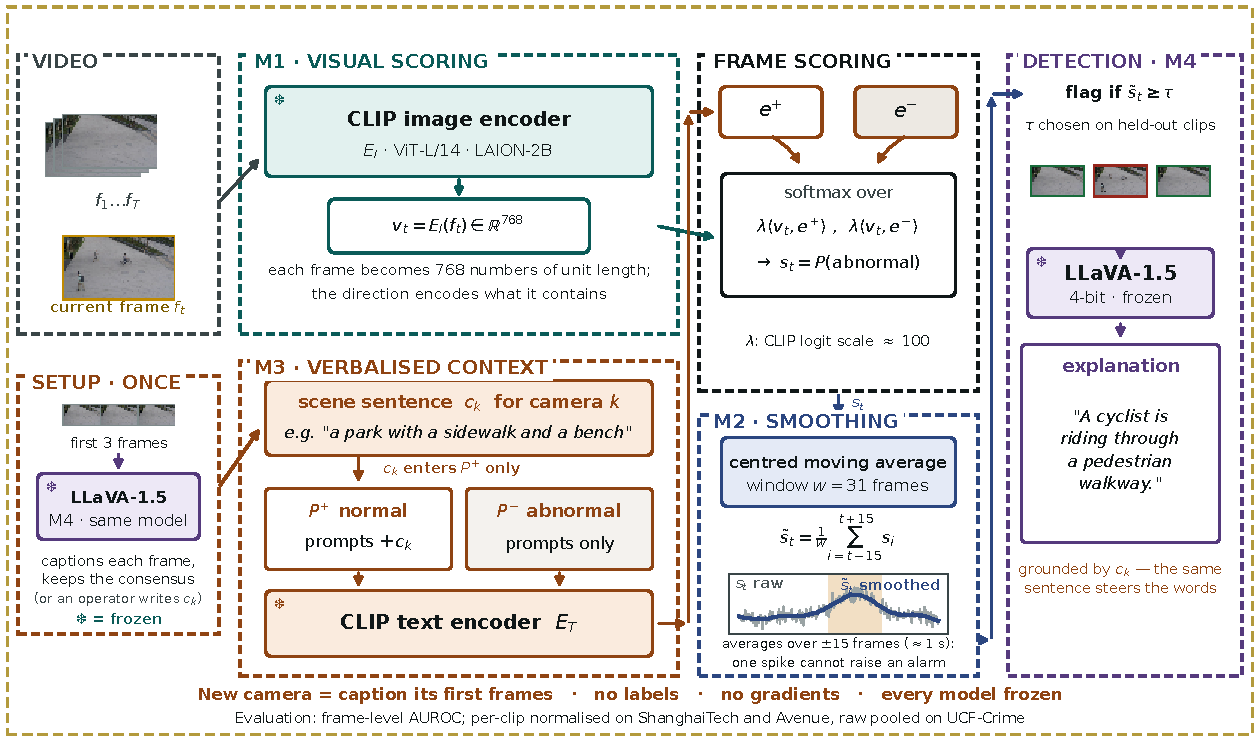
\includegraphics[width=0.92\textwidth]{dazvad_architecture}
\caption{DA-ZVAD. At setup, a frozen LLaVA captions a camera's first three
frames and the consensus caption becomes that camera's descriptor $c_k$. $c_k$
enters the normal prompt ensemble only. A frozen CLIP encoder scores each frame
against the two prompt prototypes, a moving average smooths the scores, and the
same LLaVA can explain flagged events. Nothing is trained.}
\label{fig:arch}
\end{figure*}

\textbf{M1 --- visual scoring.} A frozen CLIP ViT-L/14
encoder~\cite{radford2021clip, dosovitskiy2021vit} (LAION-2B weights) embeds
each frame as a unit vector $v_t\in\mathbb{R}^{768}$. Two prompt ensembles, a
normal set $P^{+}$ and an abnormal set $P^{-}$, are encoded and mean-pooled into
prototypes $e^{+}$ and $e^{-}$. The frame score is
\begin{equation}
s_t=\frac{\exp(\lambda\langle v_t,e^{-}\rangle)}
{\exp(\lambda\langle v_t,e^{+}\rangle)+\exp(\lambda\langle v_t,e^{-}\rangle)},
\label{eq:frame}
\end{equation}
where $\lambda=100$ is CLIP's own learned logit scale. No classifier is trained.

\textbf{M2 --- temporal smoothing.} Scores are averaged over a centred window of
$w$ frames, $\tilde s_t=\frac{1}{|W_t|}\sum_{k\in W_t}s_k$, which suppresses
isolated single-frame spikes. $w$ is the only hyperparameter of this stage.

\textbf{M3 --- verbalised context.} The descriptor $c_k$ of camera $k$ is
appended to the \emph{normal} ensemble only, e.g.\ ``$c_k$, everything is
normal''. Appending it to both ensembles reverses the effect
(Section~\ref{sec:res-sweep}).

\textbf{M4 --- reasoning.} A frozen LLaVA-1.5-7B~\cite{liu2023llava}, loaded
with 4-bit NormalFloat quantisation~\cite{dettmers2023qlora}, has two roles. At
setup it captions the first three frames of a camera, chosen by position and
never by label, and the caption closest to the other two becomes $c_k$. During
operation it can explain flagged frames; this second role has not yet been
evaluated on video.

\textbf{Context sweep.} To isolate the descriptor's contribution, the identical
pipeline is run four times varying only $c$: \texttt{none}; \texttt{generic}
(``a generic scene''); \texttt{matched} (a correct description); and
\texttt{mismatched} (an industrial description on surveillance video). The
mismatched condition is the falsifying control: if a deliberately wrong
description costs nothing, the method is not using its text. The predicted
signature was fixed before measurement.

% ---------------------------------------------------------------------
\section{Experimental Setup}

\textbf{Datasets.} Table~\ref{tab:data} lists the benchmarks. MVTec~AD is an
image-level detection baseline only; the adaptation experiments use the three
video benchmarks, which span one scene (Avenue), twelve
(ShanghaiTech) and several hundred (UCF-Crime). Fig.~\ref{fig:samples} shows
that within one ShanghaiTech camera, normal and anomalous frames differ only in
the event.

\begin{table}[t]
\caption{Datasets (test splits).}
\label{tab:data}
\centering\footnotesize
\begin{tabular}{@{}p{1.75cm}p{5.5cm}@{}}
\toprule
\textbf{Dataset} & \textbf{Content} \\
\midrule
MVTec AD~\cite{bergmann2019mvtec} & 15 categories, 1{,}725 images; baseline only \\
ShanghaiTech~\cite{liu2018shanghaitech} & Campus CCTV, 12 test views, 107 clips;
20{,}449 frames scored (every 2nd) \\
CUHK Avenue~\cite{lu2013avenue} & One campus view, 21 clips; 7{,}669 frames scored \\
UCF-Crime~\cite{sultani2018ucfcrime} & Real CCTV, 13 crime classes, 290 videos
(140 anomalous); 69{,}634 frames scored (every 16th) \\
\bottomrule
\end{tabular}
\end{table}

\begin{figure*}[t]
\centering
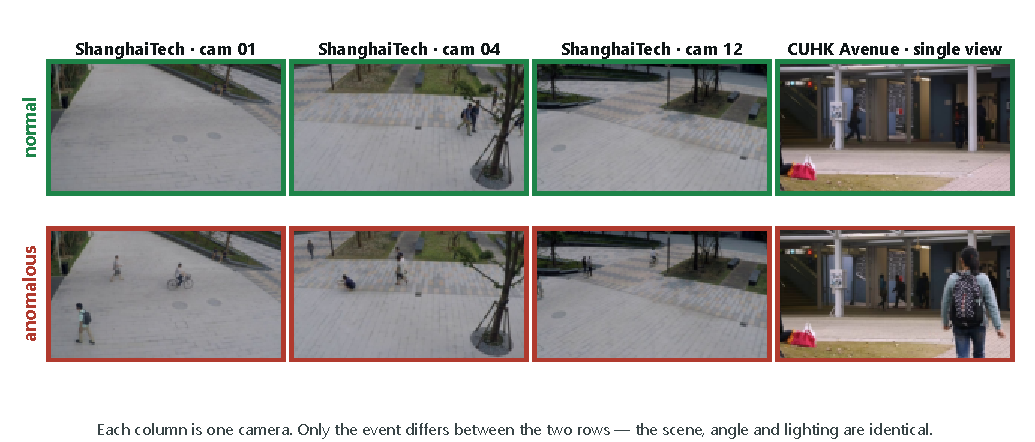
\includegraphics[width=0.82\textwidth]{fig_dataset_samples}
\caption{Normal and anomalous frames from the two campus benchmarks. Each column
is one fixed camera: scene, viewpoint and lighting are constant and only the
event differs.}
\label{fig:samples}
\end{figure*}

\textbf{Metric.} Frame-level AUROC~\cite{fawcett2006roc, bradley1997auc}. On
ShanghaiTech and Avenue each clip's scores are min--max normalised before
pooling, the protocol established with the benchmark~\cite{liu2018shanghaitech};
the step uses no labels. On UCF-Crime, half of whose videos contain no anomaly,
raw scores are pooled, the convention on that benchmark; this choice was
registered in advance.

\textbf{Implementation.} A single NVIDIA A40, PyTorch 2.3.1, CUDA 12.1. Image
embeddings are cached once per dataset so that scoring variants are evaluated in
seconds. Each run writes a manifest recording the code commit, hardware, library
versions, configuration and frame counts.

% ---------------------------------------------------------------------
\section{Results}

\subsection{Industrial baseline}
On MVTec~AD the frozen scorer reaches 88.5\% image AUROC with no training data,
against 92.4\% for a One-Class SVM~\cite{scholkopf2001oneclass} trained on the
same CLIP features. Textures average 99.5\% and objects 83.1\%: whole-image
embeddings capture global appearance changes but not small localised defects.

\subsection{ShanghaiTech: detection and the pooling protocol}
With no descriptor, the frozen scorer reaches 0.667 AUROC at $w{=}1$ and 0.707
at $w{=}31$ once clips are normalised before pooling. Pooling raw scores
instead gives 0.493 and 0.519 --- chance --- because CLIP sits at a different
score baseline under each of the twelve cameras; the same scores rank correctly
within each clip. Smoothing helps up to $w{=}31$ and falls back at $w{=}61$
(0.683), so the window has a genuine optimum.

\subsection{Context sweep: the injection point dominates}
\label{sec:res-sweep}
Table~\ref{tab:sweep} reports the sweep under two fusion rules. With the
descriptor in both ensembles the predicted order is reversed: the correct
description is worst. With it in the normal ensemble only, the predicted
signature appears: the wrong description lowers AUROC by 0.105. The
\texttt{none} column is identical in both rows, confirming that only the fusion
rule changed (Fig.~\ref{fig:sweep}).

\begin{table}[t]
\caption{Context sweep, ShanghaiTech, $w{=}31$, all 107 clips.}
\label{tab:sweep}
\centering\footnotesize
\setlength{\tabcolsep}{4pt}
\begin{tabular}{@{}lccccc@{}}
\toprule
\textbf{Fusion} & \textbf{none} & \textbf{gen.} & \textbf{match.} & \textbf{mism.} & \textbf{gap} \\
\midrule
Both sets & 0.707 & 0.670 & 0.666 & 0.695 & $-0.029$ \\
Normal only & 0.707 & 0.691 & \textbf{0.734} & 0.628 & $\mathbf{+0.105}$ \\
\bottomrule
\end{tabular}
\end{table}

\begin{figure*}[t]
\centering
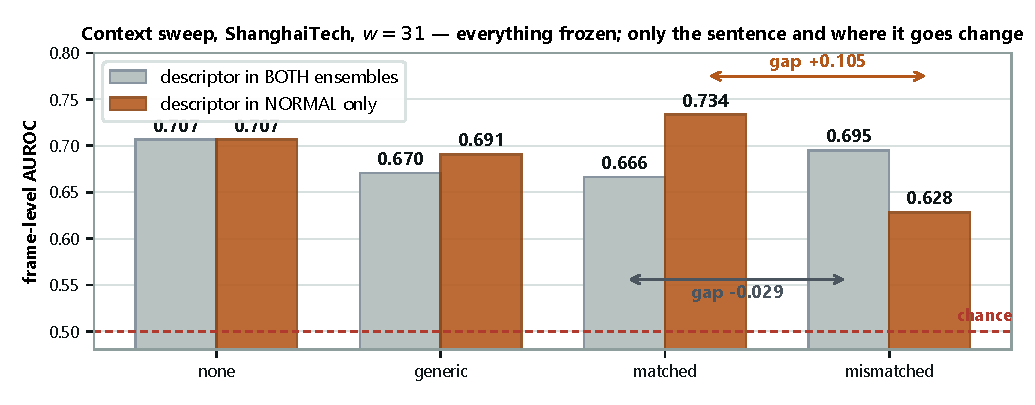
\includegraphics[width=0.78\textwidth]{fig_chart_sweep}
\caption{Table~\ref{tab:sweep} drawn: moving the descriptor from both ensembles
to the normal ensemble alone changes the matched--mismatched gap from $-0.029$
to $+0.105$.}
\label{fig:sweep}
\end{figure*}

The mechanism is prototype dilution. Each ensemble is mean-pooled, so text
appended to both enters both prototypes and draws them together: the angle
between $e^{+}$ and $e^{-}$ shrinks from $35.7^\circ$ to $25$--$26^\circ$ for
every descriptor. An accurate descriptor is the most harmful because it also
moves the pair onto the image embeddings: the mean cosine between frames and the
prototype pair rises by $+0.067$ for the matched descriptor against $+0.014$
for the generic one and $-0.017$ for the mismatched one. With normal-only
fusion, the matched descriptor instead widens the angle to $41.9^\circ$.

The positive half of the effect is weaker: the correct descriptor beats none by
$+0.027$, positive at every window but inside the $\pm0.036$ spread between data
partitions, so only its direction is claimed.

\subsection{Components and negative results}
Scored on held-out clip partitions, the language pathway alone (0.718) is not
improved by adding a motion signal (0.711) or a clip-centre normality reference
(0.645). Six modifications were tested and none helped, including quadrant-level
scoring and a prompt ensemble naming the benchmark's anomaly classes (0.486),
which re-creates the dilution above through shared vocabulary.

\subsection{Scene diversity bounds the effect}
Applied unchanged to Avenue, detection transfers (0.706 against 0.707 with no
descriptor) but the context gap falls to $+0.020$. Avenue has one camera, so
the descriptor has nothing to distinguish. Evaluating the sweep inside each
ShanghaiTech camera separately reproduces this (Table~\ref{tab:scenes},
Fig.~\ref{fig:within}): the mean within-view gap is $+0.033$, with a bootstrap
95\% interval of $[-0.005, +0.070]$ that excludes the pooled $+0.105$. Three of
the twelve test views lack enough scorable clips and are excluded.

\begin{table}[t]
\caption{Context gap against the number of scenes. ShanghaiTech and Avenue:
$w{=}31$, per-clip normalised. UCF-Crime: per-video descriptors, raw, $w{=}5$.}
\label{tab:scenes}
\centering\footnotesize
\begin{tabular}{@{}p{3.6cm}ccc@{}}
\toprule
\textbf{Evaluation} & \textbf{Scenes} & \textbf{Clips} & \textbf{Gap} \\
\midrule
Avenue & 1 & 21 & $+0.020$ \\
ShanghaiTech, within a view & 1 each & 5--34 & $+0.033$ \\
ShanghaiTech, pooled & 12 & 107 & $+0.105$ \\
UCF-Crime & $\sim$290 & 290 & $+0.096$ \\
\bottomrule
\end{tabular}
\end{table}

\begin{figure*}[t]
\centering
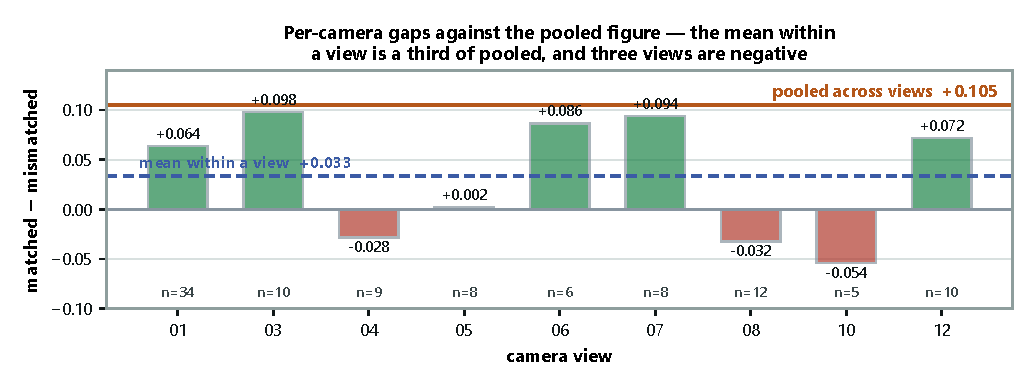
\includegraphics[width=0.78\textwidth]{fig_chart_within_view}
\caption{The context gap inside each ShanghaiTech camera view against the pooled
figure. Most views fall well short of it and three are negative.}
\label{fig:within}
\end{figure*}

\subsection{Per-camera descriptors written by the system}
If the descriptor's role is to identify the scene, twelve cameras should not
share one sentence. Table~\ref{tab:perview} gives each camera its own: written by
hand, 0.749; generated by LLaVA from each camera's first three frames, with no
human input and no labels, 0.751. The control assigns each camera another
camera's sentence --- every one a plausible campus description --- under all
eleven rotations; both per-camera sets beat every rotation, by $+0.034$ and
$+0.043$ on average (Fig.~\ref{fig:perview}). The gain over the shared sentence
is within the noise and only its direction is claimed. An earlier run chose the
frames to caption using labels (0.755); removing that changed the result by
0.004.

\begin{table}[t]
\caption{Per-camera descriptors, ShanghaiTech, $w{=}31$.}
\label{tab:perview}
\centering\footnotesize
\begin{tabular}{@{}p{5.0cm}c@{}}
\toprule
\textbf{Descriptor} & \textbf{AUROC} \\
\midrule
None & 0.707 \\
One shared sentence & 0.734 \\
Per camera, hand-written & 0.749 \\
\textbf{Per camera, generated by LLaVA} & \textbf{0.751} \\
Hand-written, swapped (mean / best of 11) & 0.715 / 0.737 \\
Generated, swapped (mean / best of 11) & 0.707 / 0.722 \\
\bottomrule
\end{tabular}
\end{table}

\begin{figure*}[t]
\centering
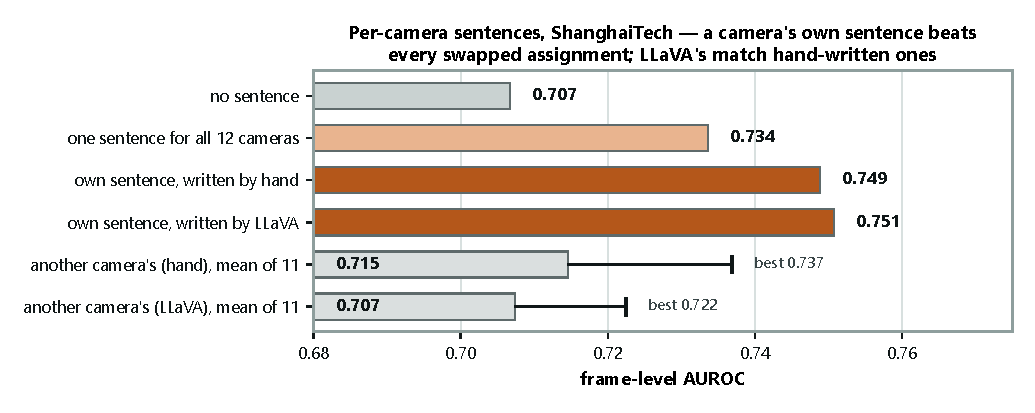
\includegraphics[width=0.78\textwidth]{fig_chart_per_camera}
\caption{Per-camera sentences beat every swapped assignment; LLaVA's sentences
match hand-written ones. The axis begins at 0.68.}
\label{fig:perview}
\end{figure*}

\subsection{UCF-Crime under pre-registered predictions}
UCF-Crime~\cite{sultani2018ucfcrime} tests the account on data it was not
developed on. Four predictions and the protocol were committed to the
repository before any score was computed. Each video's descriptor is generated by
LLaVA from its first three sampled frames; in 3 of the 140 anomalous videos the
event has already begun within them, and those captions are kept.

\begin{table}[t]
\caption{UCF-Crime, 290 videos. Raw pooled AUROC is primary.}
\label{tab:ucf}
\centering\footnotesize
\begin{tabular}{@{}p{3.9cm}cc@{}}
\toprule
\textbf{Descriptor} & \textbf{Raw} & \textbf{Normalised} \\
\midrule
None & 0.756 & 0.759 \\
Generic & 0.729 & 0.740 \\
One shared sentence & 0.813 & 0.767 \\
\textbf{Per video, LLaVA} & \textbf{0.824} & \textbf{0.789} \\
Swapped (mean / best of 20) & 0.713 / 0.779 & 0.741 / 0.784 \\
Mismatched (industrial) & 0.727 & 0.746 \\
\bottomrule
\end{tabular}
\end{table}

Table~\ref{tab:ucf} and Fig.~\ref{fig:ucf} report the result. Three predictions
held: a video's own sentence beats other videos' sentences ($+0.110$) and the
shared sentence ($+0.011$, direction only), and the correct domain beats the
wrong one ($+0.086$). The fourth, that the gap would \emph{grow} beyond
ShanghaiTech's $+0.105$ with several hundred scenes, was refuted ($+0.096$); the
claim is accordingly narrowed from ``the benefit scales with scene diversity'' to
``the benefit requires it''. Another video's sentence scores below none (0.713
against 0.756): a description of the wrong scene misleads. Under per-video
normalisation every figure is lower and the context effect is much weaker.

\begin{figure*}[t]
\centering
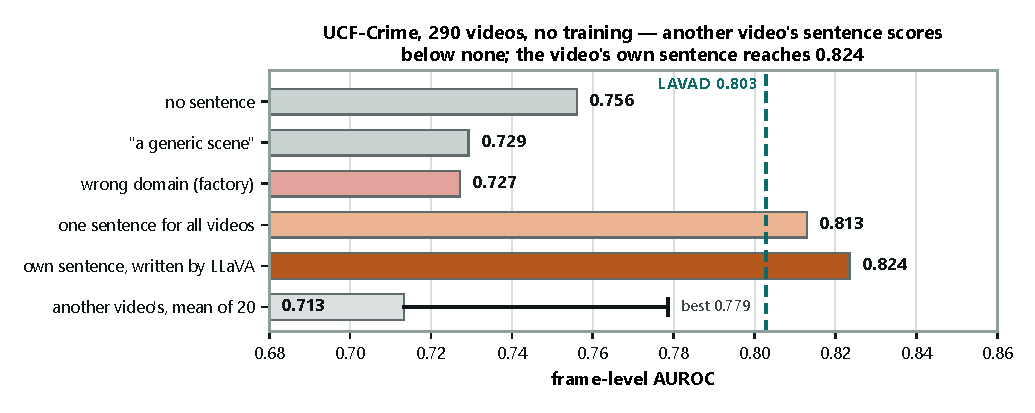
\includegraphics[width=0.78\textwidth]{fig_chart_ucf_crime}
\caption{UCF-Crime, primary metric. The dashed line is LAVAD's reported
80.28~\cite{zanella2024lavad}, a figure from another paper shown for reference.
The axis begins at 0.68.}
\label{fig:ucf}
\end{figure*}

\subsection{What the descriptor changes}
\label{sec:res-within}
The gaps above are measured with pooled AUROC, which compares frames across
videos. Judged instead only by how frames rank \emph{within} each video
(macro AUROC, invariant to any rescaling inside a clip), the ShanghaiTech
matched--mismatched gap at $w{=}5$ is $+0.006$, against $+0.100$ pooled at the
same setting. Scoring with the raw cosine margin instead of the softmax of
Eq.~\eqref{eq:frame}, which ranks frames identically within a clip, reduces the
pooled gap at $w{=}31$ to $+0.017$. The descriptor therefore acts mainly as a
near-constant shift of each video's score level --- identifying the scene and
calibrating cameras against one another --- and only weakly re-ranks frames
within a video; CLIP's large logit scale and per-clip normalisation turn that
shift into pooled-AUROC differences. This is consistent with every result above:
no effect on one camera, a smaller effect within a view, gains from per-camera
sentences, and harm from swapped ones. A full audit across all benchmarks is the
next experiment.

\subsection{Comparison with published methods}
Table~\ref{tab:sota} compares training-free methods; figures are as published
in AnyAnomaly~\cite{anyanomaly2025} (Tables~5--6), except the UCF-Crime rows
marked $^\ddagger$, from LAVAD~\cite{zanella2024lavad} (Table~1). On UCF-Crime,
the most diverse benchmark, DA-ZVAD is first of six; on the two campus
benchmarks AnyAnomaly leads. AnyAnomaly is given the benchmark's anomaly classes
as its query at evaluation, whereas DA-ZVAD receives a scene description and no
information about the anomalies. LAVAD samples every 16th frame, as here, but
cross-paper figures can differ through protocol details, so the comparison is
reported as comparable-or-better rather than as a margin.

\begin{table}[t]
\caption{Training-free methods, frame-level AUROC (\%).}
\label{tab:sota}
\centering\footnotesize
\setlength{\tabcolsep}{4pt}
\begin{tabular}{@{}lccc@{}}
\toprule
\textbf{Method} & \textbf{Ave} & \textbf{ShT} & \textbf{UCF} \\
\midrule
Zero-shot CLIP~\cite{radford2021clip} & 62.3 & 60.9 & 53.2$^\ddagger$ \\
Zero-shot ImageBind~\cite{girdhar2023imagebind} & 64.5 & 61.3 & 53.7$^\ddagger$ \\
LLaVA-1.5~\cite{liu2023llava} & 67.4 & 59.6 & 72.8$^\ddagger$ \\
Video-ChatGPT~\cite{maaz2024videochatgpt} & 76.9 & 69.1 & --- \\
LAVAD~\cite{zanella2024lavad} & --- & --- & 80.3$^\ddagger$ \\
\textbf{DA-ZVAD (ours)} & 67.7 & 73.4 & \textbf{82.4} \\
AnyAnomaly~\cite{anyanomaly2025} & \textbf{87.3} & \textbf{79.7} & 80.7 \\
\bottomrule
\end{tabular}
\end{table}

For scale, one-class methods trained on each benchmark's normal footage reach
85--91 on Avenue and 73--81 on ShanghaiTech~\cite{anyanomaly2025}; DA-ZVAD's
73.4 on ShanghaiTech is slightly above that benchmark's own baseline
(72.8)~\cite{liu2018shanghaitech}, which is trained on ShanghaiTech's training
split, at no target-data cost. On Avenue
the method trails, because its anomalies --- an object too close to the camera,
throwing, running --- are about distance and motion, which whole-frame semantic
embeddings do not capture.

% ---------------------------------------------------------------------
\section{Limitations}
\begin{itemize}
  \item The adaptation effect requires several scenes; it is absent on
        single-camera Avenue, and a registered prediction that it grows with
        scene diversity was refuted.
  \item The effect is mainly cross-camera calibration rather than within-video
        re-ranking (Section~\ref{sec:res-within}); pooled metrics are sensitive
        to score rescaling, a property of the protocol that affects other
        CLIP-based methods as well.
  \item Whole-frame embeddings at $224\times224$ cannot resolve small objects;
        patch-level scoring is untested.
  \item No validation split exists for these benchmarks; settings were chosen on
        held-out clip partitions of the test set.
  \item On UCF-Crime AUROC is computed over sampled frames, and descriptors come
        from each video's first second.
  \item The explanation role of M4 has not been evaluated on video.
\end{itemize}

% ---------------------------------------------------------------------
\section{Progress and Future Work}

Phase~1 established the concept-shift characterisation from the DA surveys and
built the frozen framework. Phase~2 measured ShanghaiTech and Avenue, diagnosed
the pooling error and the injection-point inversion, and ran the within-view
control. Phase~3 added per-camera descriptors generated by the system, the
pre-registered UCF-Crime evaluation, the prototype-direction measurement, the
within-video analysis, and a check of every cited figure against its source.

Next steps, in order: (i) a measurement audit of within-video ranking and raw
scores on all three benchmarks; (ii) XD-Violence under the same pre-registered
protocol, and UCF-Crime with scores propagated to every frame; (iii) the NWPU
Campus benchmark, whose scene-dependent anomalies directly test concept shift;
(iv) patch-level scoring and evaluation of M4's explanations.

% ---------------------------------------------------------------------
\section{Conclusion}

Domain shift in video anomaly detection is concept shift, the type the DA
literature sets aside. A fully frozen pipeline in which one sentence per camera
carries the adaptation makes that adaptation measurable, and a deliberately
wrong sentence provides a falsifying control. The sentence can be written by the
system itself, and with it the pipeline reaches 0.824 AUROC on UCF-Crime with no
training. Where the sentence enters matters more than what it says; the benefit
requires several scenes; and the effect operates mainly by putting different
cameras on a common scale. Each of these was established by an experiment that
could have failed, and one registered prediction did.

\bibliographystyle{IEEEtran}
\bibliography{references}

\end{document}
